\chapter{Наблюдения, тёмная материя и космологическое согласование}

\lectureoverview{Наблюдение приобретает смысл лишь после того, как его связывают с космологической моделью. Мы начнём с уравнения Фридмана и трёх однородных пространственных геометрий, разложим нынешний космический бюджет на излучение, материю, энергию вакуума и кривизну и восстановим, почему когда-то открытая Вселенная казалась неизбежной. Затем кривые вращения галактик обнаруживают недостающую гравитирующую материю и приводят к динамике холодного слабо взаимодействующего гало. Наконец, красное смещение, яркость и подсчёт источников превращают пробную историю расширения в наблюдаемые кривые. Старая модель «материя плюс кривизна» не работает; успешное согласование в этой лекции дают доля материи около \(0.3\), доля вакуума около \(0.7\) и очень малая кривизна.}

\section{Подставим наблюдения обратно в уравнения}

Астрономические факты нельзя интерпретировать изолированно. Сначала нам нужны уравнения, которые показывают, какие комбинации наблюдений отличают одну Вселенную от другой. Для однородной и изотропной Вселенной исходной точкой служит уравнение Фридмана,
\begin{equation}
\left(\frac{\dot a}{a}\right)^2
=
\frac{8\pi G}{3}\rho-\frac{k}{a^2}.
\label{eq:c06-friedmann}
\end{equation}
Величина
\begin{equation}
H(t)=\frac{\dot a(t)}{a(t)}
\label{eq:c06-hubble}
\end{equation}
— это \emph{функция} Хаббла. Её современное значение \(H_0\) по традиции называется постоянной Хаббла, но \(H(t)\) не является постоянной на протяжении космической истории. Когда астрономы приводят значение в километрах в секунду на мегапарсек, они имеют в виду \(H_0\).

Нормированный параметр кривизны принимает только три значения,
\begin{equation}
k\in\{+1,0,-1\},
\end{equation}
соответствующие, соответственно, сферической, плоской и гиперболической пространственной геометрии. Обычную метрику FRW можно записать в виде
\begin{equation}
ds^2=-dt^2+a(t)^2\left[dr^2+\xi(r)^2d\Omega_2^2\right],
\label{eq:c06-frw}
\end{equation}
где
\begin{equation}
\xi(r)=
\begin{cases}
\sin r, & k=+1,\\
r, & k=0,\\
\sinh r, & k=-1.
\end{cases}
\label{eq:c06-xi}
\end{equation}
Эта запись выполняет две задачи. Она объединяет три геометрии в одной метрике, а позже даёт площадь сферы и тем самым число источников в радиальной оболочке. Таким образом, выбор \(k\) и уравнение для \(a(t)\) уже задают модель с наблюдательными последствиями.

\section{Современный космический бюджет}

В обсуждаемой модели плотность энергии имеет три основных компонента: излучение, нерелятивистскую материю и энергию вакуума. Если включить кривизну в ту же строку баланса, получим
\begin{equation}
\frac{C_r}{a^4}
+\frac{C_m}{a^3}
+\Lambda
-\frac{k}{a^2}
=H^2.
\label{eq:c06-budget}
\end{equation}
Здесь \(\Lambda\) использует нормировку предыдущей лекции, \(\Lambda=(8\pi G/3)\rho_{\rm vac}\). Излучение убывает как \(a^{-4}\), материя — как \(a^{-3}\), энергия вакуума не убывает, а кривизна масштабируется как \(a^{-2}\). Кривизна не является плотностью энергии какого-либо вещества, но её постановка рядом с остальными членами делает современное ограничение прозрачным: четыре вклада должны в сумме дать \(H_0^2\).

Определим их современные доли как
\begin{equation}
\begin{aligned}
\Omega_r&=\frac{C_r/a_0^4}{H_0^2},
&\qquad
\Omega_m&=\frac{C_m/a_0^3}{H_0^2},\\
\Omega_\Lambda&=\frac{\Lambda}{H_0^2},
&
\Omega_k&=\frac{-k/a_0^2}{H_0^2}.
\end{aligned}
\label{eq:c06-omegas}
\end{equation}
Тогда
\begin{equation}
\boxed{\Omega_r+\Omega_m+\Omega_\Lambda+\Omega_k=1.}
\label{eq:c06-sum-rule}
\end{equation}
Величины \(\Omega\) — это отношения, вычисленные сегодня, а не не зависящие от времени постоянные. Заметьте также соглашение о знаке: \(k=-1\) даёт положительное \(\Omega_k\).

\subsection{Как измеряют первые члены}

Хаббл получил локальную скорость расширения, сравнивая красное смещение удаления с расстоянием. При малых \(z\) красное смещение задаёт скорость; откалиброванная яркость — расстояние. Его первое численное значение оказалось сильно ошибочным, но метод был верным. Поскольку галактики были сравнительно близкими, измерение не охватывало большую долю космической истории и могло принимать \(H\) равным его современному значению.

\begin{classroomqa}
\audiencequestion{Как яркость может определять расстояние, если собственная светимость заранее не известна?}
\lecturerresponse{В один шаг — никак. Космическая лестница расстояний начинается с параллакса близких звёзд. Переменные цефеиды в этой откалиброванной области обнаруживают соотношение период–светимость и становятся стандартными свечами на больших расстояниях. Перекрывающиеся калибровки продвигают эту лестницу дальше, а сверхновые дают лучшие свечи при космологических красных смещениях, используемых далее. Поэтому расстояние выводится из цепочки стандартов, а не из произвольного предположения, что все объекты светят одинаково. \lecturetimestamp{00:10:00--00:11:32}}
\end{classroomqa}

\begin{classroomqa}
\audiencequestion{Являются ли \(C_r\) и \(C_m\) постоянными, хотя их плотности меняются?}
\lecturerresponse{Да. Коэффициенты остаются фиксированными, тогда как множители \(a^{-4}\) и \(a^{-3}\) несут временную зависимость. Энергия вакуума постоянна, а кривизна масштабируется как \(a^{-2}\). Именно из-за этих неодинаковых степеней относительные вклады меняются от одной эпохи к другой. \lecturetimestamp{00:11:35--00:12:02}}
\end{classroomqa}

Член излучения можно измерить локально по фотонному фону. Большая его часть приходится на космический микроволновый фон, и его современная плотность энергии ничтожна по сравнению с другими важными компонентами. Нужен достаточно большой объём усреднения, но, чтобы установить, что \(\Omega_r\) сегодня пренебрежимо мало, не требуется далеко уходить вдоль прошлого светового конуса.

Видимую материю оценивают по галактикам, звёздным популяциям, водороду и межзвёздному газу. Эти методы скорее технически сложны, чем концептуально туманны: нужно определить типичное содержание звёзд и газа, просуммировать его по галактикам и усреднить по большому объёму. В лекции приводится старая грубая шкала: масса одного протона на кубический метр. Это гораздо больше плотности излучения, но всё равно поразительно разрежено.

\begin{classroomqa}
\audiencequestion{А как в этом балансе учитывается тёмная материя?}
\lecturerresponse{До неё мы сейчас дойдём, но сначала намеренно восстановим более старый вывод, основанный только на светящейся материи. Исторический порядок важен: он точно показывает, какой именно кажущийся вывод тёмная материя исправила и какой пробел она не закрыла. \lecturetimestamp{00:15:08--00:15:40}}
\end{classroomqa}

\section{Почему когда-то открытая Вселенная казалась неизбежной}

В старой картине излучение справедливо считалось пренебрежимо малым, энергия вакуума полагалась равной нулю, а под материей понимали только вещество, видимое в электромагнитном излучении. Получавшаяся оценка была примерно
\begin{equation}
\Omega_r\simeq0,
\qquad
\Omega_\Lambda=0,
\qquad
\Omega_m^{\rm luminous}\sim\frac{1}{20}\text{--}\frac{1}{30}.
\end{equation}
Тогда правило суммы, казалось, вынуждало иметь
\begin{equation}
\Omega_k\simeq1.
\end{equation}
Поскольку положительный вклад кривизны означает \(-k/a_0^2>0\), отсюда следовало \(k=-1\): открытая Вселенная с отрицательной кривизной. Эти числа — реконструкция прежнего аргумента, а не современная оценка параметров.

Чтобы истолковать масштаб кривизны, вернёмся к решению с доминированием материи
\begin{equation}
a(t)\propto t^{2/3}.
\end{equation}
Продифференцировав и разделив на \(a\), получаем
\begin{equation}
H(t)=\frac{\dot a}{a}=\frac{2}{3t}.
\label{eq:c06-matter-h}
\end{equation}
При нынешнем возрасте \(T\),
\begin{equation}
H_0\simeq\frac{2}{3T}.
\end{equation}
Тем самым хаббловское время имеет тот же порядок, что и возраст Вселенной. Сравнение с радиационно-доминированным случаем,
\begin{equation}
a(t)\propto t^{1/2},
\qquad
H(t)=\frac{1}{2t},
\end{equation}
показывает, что эта обратная пропорциональность возрасту не является особенностью пыли.

\begin{figure}[htbp]
\centering
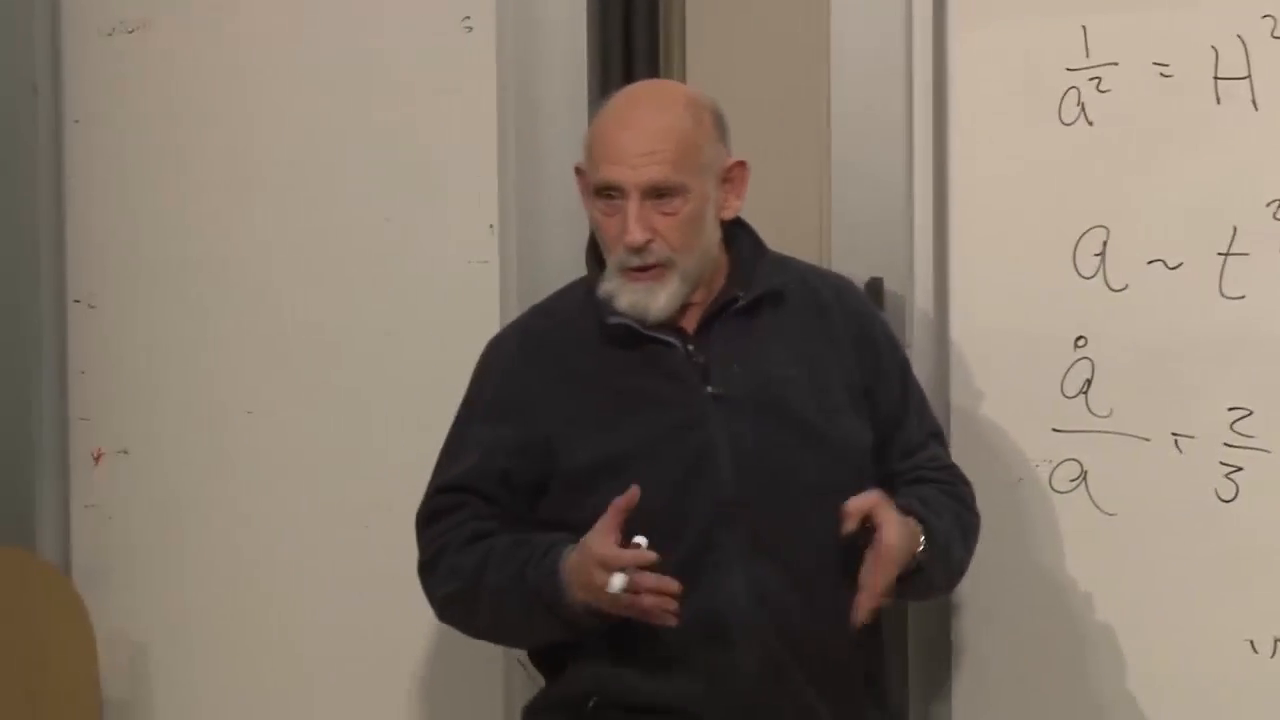
\includegraphics[width=0.72\textwidth]{lecture_06_figure_02.png}
\caption{Разбор у доски для эпохи материи. В видимой записи есть \(a\sim t^{2/3}\) и \(\dot a/a=2/(3t)\); лектор заслоняет остальную часть доски, поэтому этому кадру не приписывается никакого скрытого уравнения.}
\label{fig:c06-age-board}
\lectureframe{00:24:41.615}
\end{figure}

\begin{classroomqa}
\audiencequestion{Какие единицы имеет постоянная Хаббла и где здесь скорость света?}
\lecturerresponse{Поскольку \(H\) связывает скорость с расстоянием, у него размерность обратного времени. Его можно выражать в обратных секундах, обратных годах или в эквивалентной астрономической форме — километрах в секунду на мегапарсек. Соотношению \(H\sim1/T\) не требуется никакого дополнительного \(c\). Множитель \(c\) появляется только тогда, когда время \(T\) переводят в длину, например \(cT\). \lecturetimestamp{00:22:50--00:24:25}}
\end{classroomqa}

Исходное значение \(H_0\) у Хаббла было завышено примерно на порядок, поэтому соответствующий хаббловский возраст был слишком мал — порядка миллиарда, а не десяти миллиардов лет в округлённом сравнении лекции. Более точная калибровка исправила это число, не меняя логики того, что \(H_0^{-1}\) — космический масштаб времени.

Старый вывод о кривизне теперь записывается так:
\begin{equation}
\frac{1}{a_0^2}\sim H_0^2\sim\frac{1}{T^2}.
\end{equation}
В единицах \(c=1\) радиус кривизны \(a_0\) поэтому считался величиной порядка возраста \(T\); при восстановлении обычных единиц — порядка \(cT\). В лекции сразу же отказываются от этого как от утверждения о реальной Вселенной. Именно такой вывод получали несколькими десятилетиями ранее, отбросив члены, которые тогда считались пренебрежимо малыми.

\begin{classroomqa}
\audiencequestion{Если предполагалось, что сегодня должна доминировать кривизна, зачем использовать закон эпохи материи \(a\propto t^{2/3}\)?}
\lecturerresponse{Потому что материя масштабируется как \(a^{-3}\), тогда как кривизна — лишь как \(a^{-2}\). При меньших \(a\) доминирует материя. Кривизна могла стать важной только поздно, так что доминирование материи всё ещё описывало большую часть прошедшей истории и оставляло \(H_0\) величиной порядка \(1/T\). Полное смешанное решение поправило бы численный множитель, но не уничтожило бы аргумент о масштабе времени. \lecturetimestamp{00:49:20--00:50:17}}
\end{classroomqa}

\section{Тёмная материя из галактической динамики}

Есть два практических способа учёта материи. Один состоит в том, чтобы подсчитывать вещество, которое испускает или поглощает свет. Другой — в том, чтобы выводить массу из гравитации. Oort обнаружил аномальную галактическую динамику в начале 1930-х годов, а Zwicky обнаружил аналогичное расхождение по массе в скоплениях галактик. Данные показывали, что гравитирующей материи больше, чем светящейся. Обычное заряженное вещество излучает и сталкивается; о недостающем компоненте сначала узнали по его гравитационному действию.

\begin{classroomqa}
\audiencequestion{Включает ли светящаяся материя диффузный газ и центральные чёрные дыры?}
\lecturerresponse{Диффузный газ учитывается постольку, поскольку его количество можно вывести по его электромагнитным проявлениям. Центральная сверхмассивная чёрная дыра может быть включена в известный баланс масс, но она составляет лишь малую долю полной массы галактики и сосредоточена в центре. Она не может объяснить расхождение, сохраняющееся далеко за пределами светящегося центра. \lecturetimestamp{00:29:50--00:31:14}}
\end{classroomqa}

Рассмотрим звезду, движущуюся приблизительно по круговой орбите радиуса \(r\). Если почти вся масса \(M\) была бы сосредоточена вблизи центра галактики, то закон Ньютона дал бы
\begin{equation}
\frac{GM}{r^2}=\frac{v^2}{r},
\end{equation}
и, следовательно,
\begin{equation}
v^2=\frac{GM}{r},
\qquad
v(r)\propto r^{-1/2}.
\label{eq:c06-kepler}
\end{equation}
Это кеплеровское убывание, ожидаемое вне центрального распределения массы.

\begin{figure}[htbp]
\centering
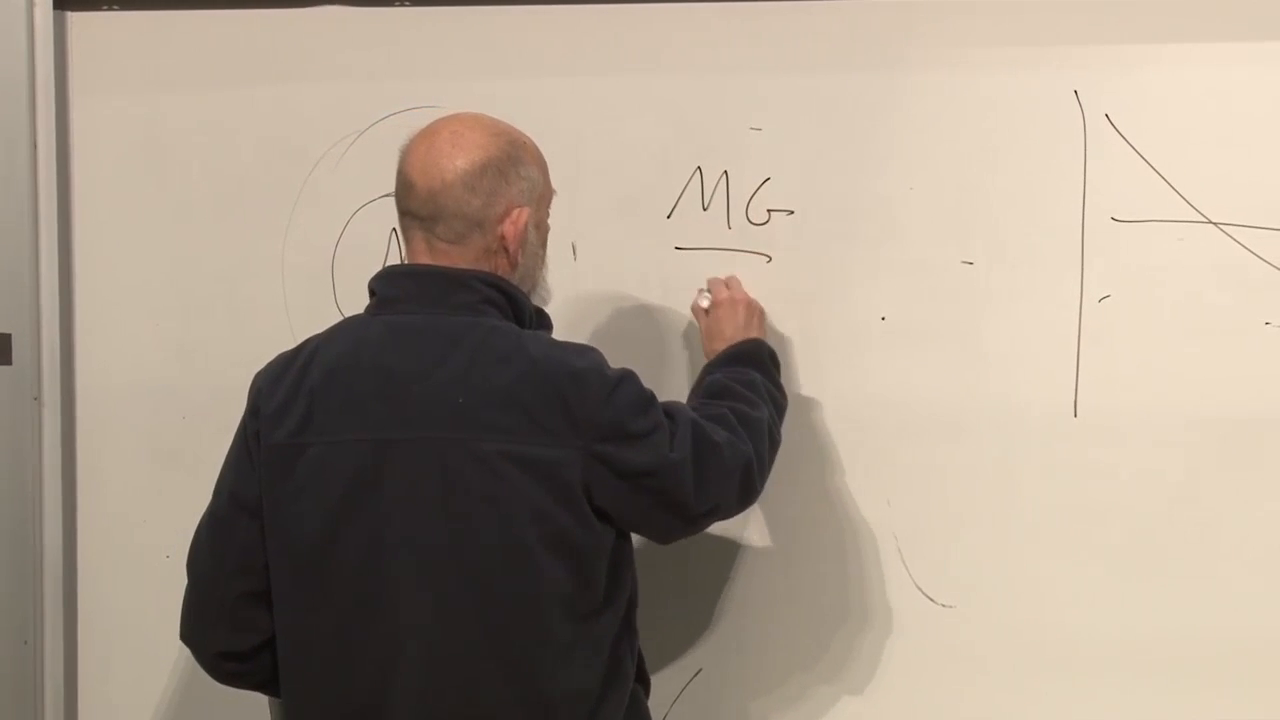
\includegraphics[width=0.78\textwidth]{lecture_06_figure_03.png}
\caption{Доска с кривой вращения в момент перехода от центральной массы к заключённой массе \(M(r)\). Видны только \(MG\), дробная черта, схема орбиты и части эскизов кривых; уравнение~\eqref{eq:c06-kepler} взято из устного вывода.}
\label{fig:c06-rotation-board}
\lectureframe{00:34:53.642}
\end{figure}

\begin{figure}[htbp]
\centering
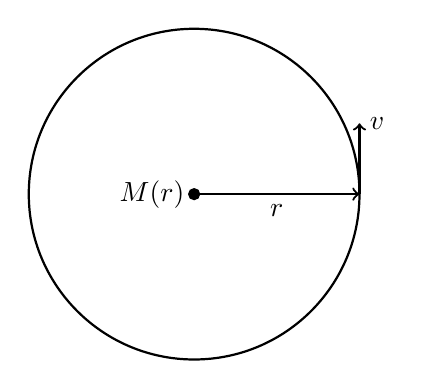
\begin{tikzpicture}[scale=1.0]
\filldraw (0,0) circle (2pt) node[left] {\(M(r)\)};
\draw[thick] (0,0) circle (2.1);
\draw[->,thick] (0,0)--(2.1,0) node[midway,below] {\(r\)};
\draw[->,thick] (2.1,0)--(2.1,0.9) node[right] {\(v\)};
\end{tikzpicture}
\caption{Построение для круговой орбиты, используемое для вывода заключённой массы по измеренной скорости вращения.}
\label{fig:c06-orbit-redraw}
\end{figure}

Наблюдаемые кривые вращения галактик так не спадают; на существенном радиальном интервале они приблизительно плоские. Заменим фиксированную центральную массу на заключённую массу \(M(r)\):
\begin{equation}
\frac{G M(r)}{r^2}=\frac{v(r)^2}{r}.
\end{equation}
Если \(v(r)\) почти постоянно, то
\begin{equation}
\boxed{M(r)\propto r.}
\label{eq:c06-enclosed-mass}
\end{equation}
Это относится к полной массе внутри радиуса \(r\), а не к локальной плотности. Гравитирующая масса продолжает расти далеко за пределами области, где сосредоточена большая часть звёздного света. Движения, перпендикулярные галактическим дискам, дополнительно указывают на приблизительно сферическое распределение: тёмное гало, а не второй тонкий диск.

\begin{classroomqa}
\audiencequestion{Есть ли простая теория, объясняющая, почему кривая вращения настолько плоская?}
\lecturerresponse{Не в рамках этого аргумента. Моделирование формирования галактик может делать такие профили естественными, но в лекции не утверждается, что существует короткий вывод. Надёжное утверждение здесь наблюдательное: почти постоянное \(v\) означает приблизительно линейный рост заключённой массы. Аккуратность этого соотношения не следует принимать за элементарное объяснение формирования галактик. \lecturetimestamp{00:35:58--00:37:33}}
\end{classroomqa}

\begin{classroomqa}
\audiencequestion{Являются ли спиральные рукава просто материальными вертушками, создаваемыми изменяющейся угловой скоростью \(v/r\)?}
\lecturerresponse{Нет, простая картина вертушки не работает. Видимая структура не обязана вращаться вместе с отдельными звёздами; среди возможных описаний — волны плотности или волны звездообразования. В лекции эта неопределённость используется, чтобы отделить надёжный вывод о гало от более сложной проблемы спиральной структуры. \lecturetimestamp{00:37:35--00:38:34; 00:47:03--00:47:47}}
\end{classroomqa}

Оцениваемая тёмная масса в несколько раз превышает светящуюся массу; в лекции приводится лишь порядок величины — множитель примерно от пяти до десяти. Гало также простирается за пределы видимой галактики. Это намеренно грубые исторические масштабы, а не точные универсальные отношения для каждой системы.

\section{Какой должна быть тёмная материя}

Почему обычная материя образует яркие компактные диски, тогда как тёмная материя остаётся в обширном гало? Светящаяся материя может терять механическую энергию благодаря электромагнитным столкновениям и излучению. После диссипации энергии гравитация может стянуть её в более плотную конфигурацию. Тёмная материя, по-видимому, электрически нейтральна и взаимодействует гораздо слабее. Её частицы обращаются в гало, почти не сталкиваясь и не излучая, поэтому даже за миллиарды лет они не теряют достаточно энергии, чтобы осесть в светящемся диске. Гравитационное излучение от галактического движения слишком слабо, чтобы служить альтернативным механизмом охлаждения.

\begin{classroomqa}
\audiencequestion{Означает ли слабое взаимодействие, что тёмная материя подчиняется иному закону гравитации?}
\lecturerresponse{Нет. Предполагается, что она гравитирует обычным образом. Слабое взаимодействие здесь означает отсутствие негравитационных столкновений и электромагнитного излучения или их сильное подавление. Две тёмные частицы всё равно гравитационно притягиваются; это притяжение организует гало, но не обеспечивает эффективной диссипации орбитальной энергии. \lecturetimestamp{00:42:36--00:43:35}}
\end{classroomqa}

\begin{classroomqa}
\audiencequestion{Какие наблюдения показывают, что это — не просто особенность одной галактической кривой вращения?}
\lecturerresponse{Свидетельства проявляются на нескольких масштабах: движение звёзд внутри галактик, движение перпендикулярно плоскостям галактик, взаимодействия между галактиками и динамика целых скоплений галактик. Примеры Oort и Zwicky были разными проявлениями одной и той же проблемы недостающей гравитации. \lecturetimestamp{00:42:00--00:42:36}}
\end{classroomqa}

\begin{classroomqa}
\audiencequestion{Должна ли тёмная материя скапливаться вокруг чёрных дыр и галактических центров?}
\lecturerresponse{Она действительно становится плотнее по мере приближения к гравитационному центру, но последовательность событий, вероятно, обратна картине, в которой гало формируется вокруг заранее существовавшей чёрной дыры. Тёмные гало сформировали большие гравитационные потенциальные ямы; затем в них падала барионная материя и образовывала галактики, звёзды и центральные чёрные дыры. Чёрная дыра составляет малую часть массы. Тем не менее поиски продуктов аннигиляции направлены на галактический центр, потому что там ожидается более высокая плотность тёмной материи. \lecturetimestamp{00:43:36--00:45:43}}
\end{classroomqa}

\begin{classroomqa}
\audiencequestion{Является ли тёмная материя газом, пылью, компактными сгустками или отдельными частицами? Могут ли некоторые из них быть захвачены вблизи Солнца?}
\lecturerresponse{Её микроскопическая природа неизвестна, но обычная пыль связана электромагнитными силами — именно такого рода взаимодействий, по-видимому, тёмной материи недостаёт. Поэтому стандартное представление состоит в том, что это разреженная популяция отдельных частиц. Некоторые могут быть гравитационно сконцентрированы вблизи Солнца, однако их плотность слишком мала, чтобы конкурировать с солнечной гравитацией или возмущать динамику планет. \lecturetimestamp{00:45:43--00:47:02; 00:58:41--00:59:29}}
\end{classroomqa}

Второе основное требование состоит в том, чтобы тёмная материя образовывала скопления. Горячая популяция со случайными релятивистскими скоростями сопротивляется гравитационной агрегации; холодная популяция может падать в потенциальные ямы. Обычные лёгкие нейтрино вели бы себя как горячая тёмная материя и не дают требуемого основного галактического компонента. В этом контексте термин \emph{холодная} означает нерелятивистский режим в локальной космологической системе отсчёта, а не буквально лабораторную нулевую температуру.

\begin{classroomqa}
\audiencequestion{Накладывает ли требование, чтобы тёмная материя была холодной и образовывала скопления, ограничения на диапазон её масс?}
\lecturerresponse{Это зависит от квантовой статистики и истории образования. Очень лёгкие фермионы не могут все находиться в одном медленном состоянии, и на них накладываются сильные ограничения. Очень лёгкие бозоны могут занимать когерентное бозе-конденсированное состояние; в лекции в качестве примера приводятся аксионы. Либо более тяжёлые слабо взаимодействующие частицы могут быть холодными и без конденсации. Таким образом, этот аргумент не даёт единственной, не зависящей от модели границы для массы. \lecturetimestamp{00:53:17--00:54:52; 00:56:42--00:58:05}}
\end{classroomqa}

\begin{classroomqa}
\audiencequestion{Должны ли были ускорители уже обнаружить эти частицы?}
\lecturerresponse{Только при дополнительных предположениях. Если частицы имеют сечения порядка слабого взаимодействия и массы в пределах досягаемости ускорителей, их рождение в коллайдерах может быть возможным. Высказанное в лекции ожидание скорой информации было явно спекулятивным и исторически обусловленным. Частица может, напротив, быть слишком тяжёлой или взаимодействовать слишком слабо для имеющихся экспериментов. \lecturetimestamp{00:54:52--00:55:54}}
\end{classroomqa}

\begin{classroomqa}
\audiencequestion{Может ли тёмная материя просто находиться в ненаблюдаемом дополнительном измерении?}
\lecturerresponse{В этом обсуждении никакой такой механизм не требуется. Тёмная материя уже наблюдается гравитационно и может просто состоять из необычных частиц, почти не взаимодействующих с обычным веществом. Называть взаимодействие слабым — не то же самое, что помещать частицы вне наблюдаемого пространства-времени. \lecturetimestamp{00:55:54--00:56:41}}
\end{classroomqa}

Логической альтернативой является модификация гравитации, а не добавление ненаблюдаемой материи. В лекции считается, что в то время никакая сопоставимо простая модификация не объясняла данные на всех существенных масштабах, сохраняя при этом проверенные законы для Солнечной системы. Поэтому предпочтительна интерпретация в терминах частиц, но её микрофизика остаётся неизвестной.

\section{Тёмная материя не замыкает старый баланс}

Тёмная материя увеличивает вклад материи в несколько раз, но старое расхождение между светящейся материей и \(H_0^2\) было порядка двадцати пяти. Поэтому она сужает разрыв, не приводя к выполнению
\begin{equation}
\frac{C_m}{a_0^3}=H_0^2.
\end{equation}
В рамках старой картины без \(\Lambda\) по-прежнему требовался положительный член в балансе кривизны и, следовательно, \(k<0\). В такой открытой модели не было ничего логически противоречивого; суть в том, что сама по себе тёмная материя не выбирала современный ответ.

\begin{classroomqa}
\audiencequestion{Что космологи в действительности думали о кривизне до современного подбора параметров?}
\lecturerresponse{Имевшиеся данные были запутанными, и прежнее предпочтение замкнутой, ограниченной Вселенной иногда вступало в противоречие с балансом вещества. После того как старые предположения были последовательно объединены, естественным выводом оказалась отрицательная кривизна. Этот исторический консенсус всё же оставался предварительным, поскольку ни тёмная материя, ни энергия вакуума ещё не были надёжно включены так, как сегодня. \lecturetimestamp{00:50:17--00:51:50}}
\end{classroomqa}

Поэтому мы должны проверять модель-кандидат, а не заключать о её истинности по одной строке баланса. Модель состоит из выбора кривизны \(k\) и истории расширения \(a(t)\), или, эквивалентно, из набора уравнений состояния компонент и современных параметров, по которым вычисляется \(a(t)\). Прежний кандидат — это вещество плюс отрицательная кривизна при пренебрежимо малом излучении и без космологической постоянной.

\section{Переход от геометрии к наблюдаемым величинам}

\subsection{Число источников и яркость в замороженной геометрии}

Временно пренебрежём космической эволюцией. В однородной Вселенной число источников в сопутствующей оболочке пропорционально её площади:
\begin{equation}
dN\propto \xi(r)^2\,dr.
\label{eq:c06-shell-count}
\end{equation}
Следовательно,
\begin{equation}
dN\propto
\begin{cases}
\sin^2r\,dr, & k=+1,\\
r^2\,dr, & k=0,\\
\sinh^2r\,dr, & k=-1.
\end{cases}
\end{equation}
При больших \(r\) случай отрицательной кривизны растёт как \(\sinh^2r\sim e^{2r}\), гораздо быстрее, чем плоский закон \(r^2\). Поэтому отрицательная кривизна предсказывает аномально быстрое увеличение числа источников с расстоянием.

Та же площадь определяет принимаемый поток. В плоском статическом пространстве стандартный источник даёт
\begin{equation}
F\propto\frac{1}{r^2}.
\end{equation}
В гиперболическом пространстве сфера, по которой распространяется излучение, растёт быстрее, поэтому поток убывает быстрее. В лекции эту наблюдаемую величину иногда называют светимостью; здесь \(F\) обозначает яркость или поток, тогда как собственная светимость относится к источнику. Поэтому число источников и яркость вместе позволяют различать пространственные геометрии.

\subsection{Красное смещение и прошлый световой конус}

Реальная Вселенная эволюционирует, и смотреть всё дальше в пространство значит смотреть всё дальше назад во времени. Свет, испущенный в момент \(t_{\rm em}\), растягивается, пока масштабный фактор растёт от \(a(t_{\rm em})\) до \(a_0\):
\begin{equation}
1+z
=\frac{\lambda_{\rm obs}}{\lambda_{\rm em}}
=\frac{a_0}{a(t_{\rm em})}.
\label{eq:c06-redshift}
\end{equation}
Эквивалентно,
\begin{equation}
z=\frac{\lambda_{\rm obs}}{\lambda_{\rm em}}-1.
\end{equation}
Разные точки на нашем прошлом световом конусе одновременно соответствуют разным сопутствующим радиусам и разным временам испускания. Расширение меняет длину волны; доплеровский и гравитационный сдвиги — другие физические механизмы, но здесь рассматривается именно эффект космологического расширения.

\begin{classroomqa}
\audiencequestion{Почему в определение \(z\) входит минус единица?}
\lecturerresponse{Это историческое соглашение, выбранное так, чтобы для источника без смещения было \(z=0\). Физически непосредственный коэффициент растяжения — \(1+z=\lambda_{\rm obs}/\lambda_{\rm em}\). \lecturetimestamp{01:10:11--01:10:45}}
\end{classroomqa}

Для радиального света \(d\Omega_2=0\), и он удовлетворяет условию \(ds^2=0\). Уравнение~\eqref{eq:c06-frw} поэтому даёт
\begin{equation}
dt^2=a(t)^2dr^2.
\end{equation}
Для входящего луча, прослеженного назад от нас,
\begin{equation}
dt=-a(t)\,dr,
\qquad
\frac{dr}{dt}=-\frac{1}{a(t)}.
\label{eq:c06-null-ray}
\end{equation}
Знак минус означает, что большему сопутствующему радиусу соответствует более раннее время вдоль луча. Как только \(a(t)\) известно, это уравнение определяет \(r(t)\).

\subsection{Число на единицу красного смещения}

Наблюдатель может подсчитывать стандартные источники в интервале красного смещения от \(z\) до \(z+dz\). Начнём с уравнения~\eqref{eq:c06-shell-count} и продифференцируем уравнение~\eqref{eq:c06-redshift} вдоль прошлого светового луча:
\begin{equation}
dz=-\frac{a_0}{a^2}\,da
=-\frac{a_0}{a^2}\dot a\,dt.
\end{equation}
Используя \(dt=-a\,dr\),
\begin{equation}
dz=\frac{a_0}{a}\dot a\,dr
=(1+z)\dot a\,dr.
\end{equation}
Отсюда
\begin{equation}
dr=\frac{dz}{(1+z)\dot a},
\end{equation}
и при фиксированной сопутствующей плотности источников
\begin{equation}
\boxed{
\frac{dN}{dz}
\propto
\frac{\xi(r)^2}{(1+z)\dot a}
}.
\label{eq:c06-dndz}
\end{equation}
В живом выводе знаки и множители проверяются не один раз; уравнения~\eqref{eq:c06-null-ray} и \eqref{eq:c06-redshift} однозначно фиксируют результат.

\begin{figure}[htbp]
\centering
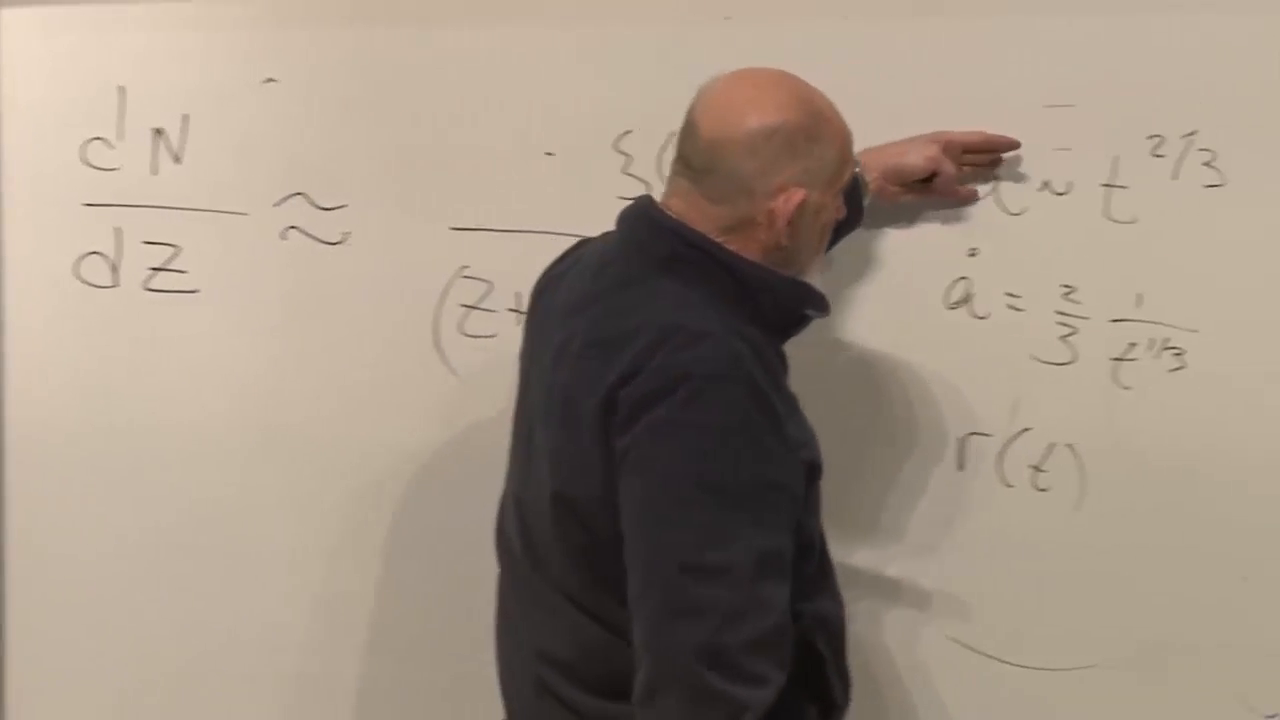
\includegraphics[width=0.84\textwidth]{lecture_06_figure_05.png}
\caption{Записанное на доске соотношение между \(dN/dz\) и функциями модели. Левая часть, а справа \(a\sim t^{2/3}\), \(\dot a\) и \(r(t)\), видны, тогда как лектор заслоняет часть знаменателя; уравнение~\eqref{eq:c06-dndz} независимо установлено выше.}
\label{fig:c06-dndz-board}
\lectureframe{01:22:24.114}
\end{figure}

Пока модель не выбрана, дальше вычислять нечего. Заданная \(a(t)\) определяет \(\dot a(t)\), уравнение~\eqref{eq:c06-null-ray} определяет \(r(t)\), а уравнение~\eqref{eq:c06-redshift} позволяет выразить любую величину через \(z\). Разные уравнения состояния порождают разные функции \(dN/dz\) и \(F(z)\). Именно поэтому наблюдения позволяют различать модели.

\section{От пробных параметров к наилучшему согласованию}

Процедура проста:
\begin{equation}
(\Omega_r,\Omega_m,\Omega_\Lambda,\Omega_k)
\longrightarrow
a(t)
\longrightarrow
\left\{F(z),\frac{dN}{dz}\right\}.
\label{eq:c06-fit-pipeline}
\end{equation}
Выберите современные параметры, решите уравнение Фридмана, проследите распространение радиального светового луча, вычислите яркость и число источников как функции красного смещения и сравните кривые с данными. Если сравнение оказывается неудачным, этот набор параметров отвергается. Вместе эти две наблюдаемые величины ограничивают как историю расширения, так и пространственную геометрию.

\begin{figure}[htbp]
\centering
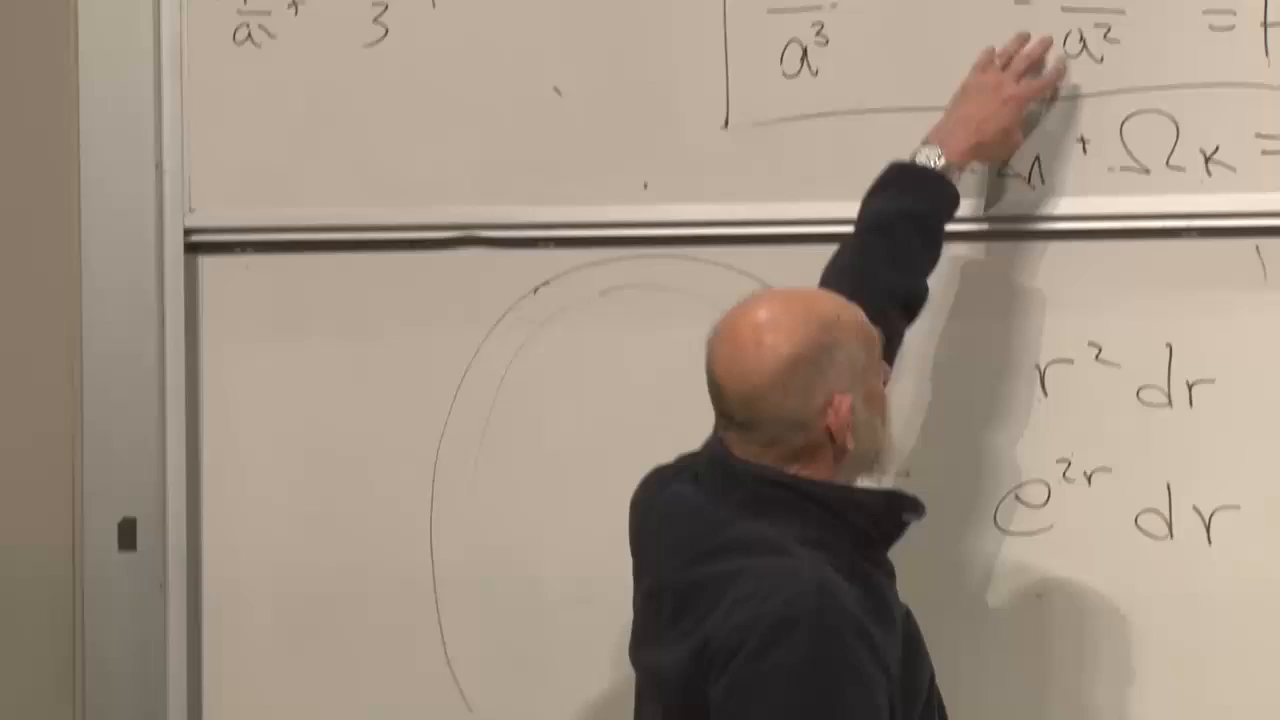
\includegraphics[width=0.84\textwidth]{lecture_06_figure_06.png}
\caption{Старая модель вещества с кривизной на верхней доске и плоский и гиперболический множители оболочки \(r^2dr\) и \(e^{2r}dr\) на нижней. Части уравнения Фридмана закрыты, поэтому этот кадр служит подтверждающим свидетельством, а не источником уравнения.}
\label{fig:c06-old-model-board}
\lectureframe{01:24:27.863}
\end{figure}

Старая модель,
\begin{equation}
H^2=\frac{C_m}{a^3}-\frac{k}{a^2},
\qquad k=-1,
\end{equation}
не проходит ни зависимость яркости от красного смещения, ни тест по числу источников. Сверхновые обеспечивают наиболее полезные стандартные свечи в соответствующем диапазоне красных смещений. Успешный набор параметров в лекции таков:
\begin{equation}
\boxed{
\Omega_r\simeq0,\qquad
\Omega_m\simeq0.3,\qquad
\Omega_\Lambda\simeq0.7,\qquad
\Omega_k\simeq0
}.
\label{eq:c06-best-fit}
\end{equation}
Здесь вещество включает светящуюся и тёмную материю. Эти значения соответствуют подбору параметров, актуальному на момент лекции; устойчивый вывод состоит в методе подбора и в необходимости доминирующего неразбавляющегося компонента, а не в последней приведённой десятичной цифре.

\subsection{Вопросы о том, что измеряется, а что подбирается}

\begin{classroomqa}
\audiencequestion{Предполагалось ли уже \(\Lambda\), когда обсуждалась старая модель открытой Вселенной?}
\lecturerresponse{Нет. В первой части намеренно была реконструирована более старая модель с \(\Lambda=0\). Значения в уравнении~\eqref{eq:c06-best-fit} описывают более позднее, современное согласование. Старый кандидат не был молча исправлен; его проверили по \(F(z)\) и \(dN/dz\), и он не прошёл проверку. \lecturetimestamp{01:26:45--01:27:07}}
\end{classroomqa}

\begin{classroomqa}
\audiencequestion{Как получают \(\Omega_\Lambda\), если энергия вакуума не измеряется напрямую, как локальное вещество?}
\lecturerresponse{Начните с пробных наборов параметров. Каждый набор задаёт решение Фридмана и тем самым предсказанные функции \(F(z)\) и \(dN/dz\). Сравните эти предсказания с наблюдениями, отбросьте плохие согласования и сохраните наилучшую область пространства параметров. Число \(0.7\) — это вывод из согласования, а не прямое считывание с измерителя энергии вакуума. \lecturetimestamp{01:27:08--01:29:59; 01:31:57--01:33:40}}
\end{classroomqa}

\begin{classroomqa}
\audiencequestion{Откуда берётся современный масштабный фактор \(a_0\)?}
\lecturerresponse{Нормировка \(a\) отчасти условна, но завершённая модель, привязанная к \(H_0\), задаёт нынешний физический масштаб кривизны при \(k\ne0\). Как только модель согласована с наблюдаемыми величинами красного смещения, её функция \(a(t)\) указывает нынешний момент и соответствующий масштаб. \lecturetimestamp{01:29:59--01:30:42}}
\end{classroomqa}

\begin{classroomqa}
\audiencequestion{Искажает ли взгляд на миллиарды лет в прошлое согласование, основанное на сегодняшних параметрах?}
\lecturerresponse{Такое заглядывание в прошлое — не искажение; это и есть сигнал. Сегодняшние параметры подставляются в уравнение Фридмана, которое разворачивает их в полную \(a(t)\). Предсказанный световой конус уже учитывает то, что при меньших \(a\) вещество было важнее, а достаточно далеко в прошлое доминирует излучение. Модель, игнорирующая эту эволюцию, не согласовалась бы с данными. \lecturetimestamp{01:30:43--01:31:55}}
\end{classroomqa}

\begin{classroomqa}
\audiencequestion{Какие современные величины измеряются сравнительно непосредственно?}
\lecturerresponse{Плотность излучения измерена и сегодня пренебрежимо мала. Параметр Хаббла измеряется из соотношения расстояние—красное смещение. Полная плотность вещества, включая светящуюся и тёмную материю, определяется по гравитации и делится на критическую плотность \(3H_0^2/(8\pi G)\), чтобы получить \(\Omega_m\). Оставшаяся свобода на поздних стадиях в основном связана с энергией вакуума и кривизной. \lecturetimestamp{01:33:40--01:35:32}}
\end{classroomqa}

\begin{classroomqa}
\audiencequestion{Если и \(\Omega_\Lambda\), и \(\Omega_k\) неизвестны, почему после фиксации \(\Omega_m\) остаётся только один независимый пробный параметр для поздней эпохи?}
\lecturerresponse{Потому что уравнение~\eqref{eq:c06-sum-rule} накладывает одно ограничение. При пренебрежимо малом \(\Omega_r\) и измеренном \(\Omega_m\) выбор пробного \(\Omega_\Lambda\) фиксирует оставшееся \(\Omega_k=1-\Omega_m-\Omega_\Lambda\). То же самое одномерное семейство можно параметризовать и кривизной. Например, \(\Omega_\Lambda=0.4\) и \(\Omega_k=0.3\) — допустимый пробный вариант при \(\Omega_m=0.3\); он отвергается только потому, что его предсказанные кривые плохо согласуются с данными, а не потому, что правило суммы его запрещает. \lecturetimestamp{01:35:33--01:39:09}}
\end{classroomqa}

\begin{classroomqa}
\audiencequestion{Как может \(k\) принимать только \(+1,0,-1\), тогда как \(\Omega_k\) меняется непрерывно, и правильны ли размерности?}
\lecturerresponse{Дискретная величина \(k\) фиксирует только знак и нормированную геометрию. Непрерывный радиус кривизны заключён в \(a_0\), поэтому \(-k/(a_0^2H_0^2)\) может принимать континуум значений. В единицах \(c=1\) обратная длина и обратное время имеют одинаковые размерности; при восстановлении обычных единиц появляются требуемые степени \(c\). \lecturetimestamp{01:39:10--01:40:07}}
\end{classroomqa}

\begin{classroomqa}
\audiencequestion{Предполагает ли метод подсчёта однородность и изотропию, хотя популяции галактик эволюционируют?}
\lecturerresponse{Он предполагает пространственную однородность и изотропию на достаточно больших срезах, и эти симметрии можно проверять, сравнивая разные направления при одном и том же красном смещении. Эволюция источников — отдельный вопрос: популяции в разные эпохи не обязаны быть одинаковыми, поэтому в практических анализах моделируют отбор и эволюцию, а не делают вид, будто численная плотность навечно фиксирована. В простом выводе сначала выделяют геометрический множитель, а уже потом добавляют эти уточнения. \lecturetimestamp{01:40:08--01:41:08}}
\end{classroomqa}

\section{Доли плотности эволюционируют}

Уравнение~\eqref{eq:c06-budget} справедливо в любой момент времени, но величины \(\Omega\) в уравнении~\eqref{eq:c06-omegas} были определены для настоящего времени. Их зависящие от времени аналоги меняются, поскольку четыре члена содержат разные степени \(a\). В далёком прошлом,
\begin{equation}
\Omega_r(t)\longrightarrow1.
\end{equation}
Поскольку излучение разрежается быстрее, материя приближается к доминированию. Позже и сама материя разрежается, тогда как \(\Lambda\) остаётся постоянной, так что в далёком будущем,
\begin{equation}
\Omega_\Lambda(t)\longrightarrow1.
\end{equation}
Поэтому доля материи сначала мала, в эпоху материи становится близкой к единице, а после того, как начинает доминировать энергия вакуума, снова падает. Кривизна, если она ненулевая, в конце концов тоже уступает положительной постоянной \(\Lambda\).

\begin{classroomqa}
\audiencequestion{Означает ли малая нынешняя доля кривизны, что Вселенная по мере расширения становится более плоской?}
\lecturerresponse{Физический масштаб кривизны растёт вместе с \(a\), а по отношению к положительной космологической постоянной вклад кривизны \(a^{-2}\) становится всё менее важным. Именно в этом смысл выражения \emph{чем больше, тем площе}. Это не меняет дискретную топологическую метку \(k\); речь лишь о том, что локальная кривизна и относительная динамическая значимость кривизны уменьшаются. \lecturetimestamp{01:47:13--01:47:42}}
\end{classroomqa}

\begin{classroomqa}
\audiencequestion{Показывала ли подогнанная модель необъяснённые систематические остаточные отклонения, и насколько точным было это утверждение?}
\lecturerresponse{В лекции говорится, что на том уровне не было известно ни о каких систематических сбоях этой схемы, и её характеризуют как прецизионную космологию примерно на уровне процента, а не десятой или сотой доли процента. Это историческое утверждение, и его не следует переиначивать в современную оценку погрешности, как если бы оно было вневременным. \lecturetimestamp{01:45:40--01:46:19}}
\end{classroomqa}

\begin{classroomqa}
\audiencequestion{Можно ли проверять пространственную кривизну прямой триангуляцией, а не только по яркости сверхновых и подсчётам?}
\lecturerresponse{Да. Угловая структура космического микроволнового фона задаёт стандартный физический масштаб и тем самым большой космический треугольник. Одни только данные по сверхновым не давали того полного утверждения о кривизне на процентном уровне, которое прозвучало в лекции; их объединение с геометрией микроволнового фона сделало проверку более строгой. Этому посвящена следующая лекция. \lecturetimestamp{01:46:19--01:47:12}}
\end{classroomqa}

\section{Что следует запомнить}

Главный вывод — не перечень из четырёх чисел. Это метод. Набор космологических параметров задаёт \(a(t)\); затем метрика предсказывает распространение света, яркость источников и число источников. Такое согласие проверяет как выбранные параметры, так и фридмановскую схему, которая их связывает. Нет никаких оснований ожидать, что произвольный набор обязательно подойдёт.

Старая модель со светящейся материей и отрицательной кривизной оказалась несостоятельной. Тёмная материя исправила состав гравитирующего вещества, но сама по себе не замкнула старый фридмановский баланс. Для успешной подгонки на момент лекции требовалось приблизительно
\begin{equation}
\Omega_m\simeq0.3,
\qquad
\Omega_\Lambda\simeq0.7,
\qquad
\Omega_k\simeq0,
\end{equation}
причём точность определения кривизны существенно зависела от микроволнового фона. Модель убедительна, потому что несколько независимых наблюдений, интерпретированных в рамках одной динамической теории, сходятся в одной и той же области пространства параметров.
